\documentclass[11pt]{article}

% bioRxiv-compatible packages
\usepackage[utf8]{inputenc}
\usepackage[T1]{fontenc}
\usepackage{amsmath,amssymb}
\usepackage{graphicx}
\usepackage{float}
\graphicspath{{../../figures/}}
\usepackage[margin=1in]{geometry}
\usepackage{natbib}
\usepackage{booktabs}
\usepackage{multirow}
\usepackage[hidelinks]{hyperref}
\usepackage{xcolor}
\usepackage{setspace}
\usepackage{textcomp}

\onehalfspacing

\title{Four Biological Mechanisms Predict ITP Sex Differences\\from Male Data Alone}
\author{Silmon James Biggs\\[0.3em]
\normalsize Longrun Bio\\
\normalsize \texttt{james@longrun.bio}}
\date{}

\begin{document}

\maketitle

\begin{abstract}
Most longevity compounds tested by the NIA Interventions Testing Program work better in male mice than female mice, except rapamycin, which works better in females. After 20 years and 54 compounds, no quantitative model has predicted the direction and magnitude of these sex differences. We built a mechanistic model of four coupled aging subsystems, each tracking a different kind of biological damage, and calibrated it to six male ITP results (6 free parameters). We then asked: can four sex-specific biological mechanisms, each taken from prior published experiments and none fitted to female data, predict all six female outcomes? They can, with 1.3 percentage point mean absolute error (MAE). The model also predicts the rapamycin + acarbose combination outcome (+33.5\% predicted vs.\ +34\% observed) without fitting to that result, correctly identifying sub-additivity from shared pathway saturation. Where the model errs, it errs informatively: the opposite mispredictions for acarbose and canagliflozin point to a second, sex-independent canagliflozin pathway (FGF21/ketogenesis) that the single-AMPK model does not capture. This is a testable hypothesis the model generates, not one it was designed to test.
\end{abstract}

% ============================================================
\section{Introduction}
% ============================================================

The biology of aging has attracted sustained theoretical attention for more than a century, producing a vast literature, remarkable more for its breadth than for its predictive power. The distinction between a theory of aging causation and a quantitative model of aging interventions is the difference between explaining \emph{why} an organism dies and predicting \emph{when}. Reliability theory \citep{Gavrilov2001} makes one piece of the problem precise: organisms are series systems that fail when any one critical subsystem reaches its threshold. The consequence is that fixing one failure mode while leaving others intact produces gains proportional to that mode's contribution and no more. The remaining modes do not vanish; they wait.

The most conspicuous unexplained pattern in 20 years of ITP data is that most longevity compounds work better in males, except rapamycin, which works better in females. Jiang et al.\ \citep{Jiang2025} documented the pattern across 54 compounds and 164 trials, confirming it is systematic, not compound-specific. Garratt \citep{Garratt2020} proposed qualitative mechanisms (pharmacokinetics, hormonal substrates, baseline pathway differences) but none were combined into a model that makes quantitative predictions.

Here we describe the Extensible Longevity Model (ELM): a system of ordinary differential equations that tracks four aging subsystems (mitochondrial heteroplasmy, DNA damage, epigenetic drift, and cellular senescence) coupled through NAD$^+$ metabolism and SASP signaling. These correspond to a subset of the Hallmarks of Aging \citep{LopezOtin2013,LopezOtin2023}; the ELM attempts to put calibrated numbers on the subset that is experimentally tractable with current ITP data.

The four subsystems are not independent. They are coupled through shared molecular intermediates, most centrally NAD$^+$, whose availability governs DNA repair (via PARP1), mitophagy (via SIRT1/FOXO3), and epigenetic stability (via EZH2). A drug that raises NAD$^+$ can partially address multiple subsystems simultaneously; conversely, two drugs that both raise NAD$^+$ may show diminishing returns when combined.

The model is calibrated to six male ITP lifespan results. Four sex-specific mechanisms, each drawn from independent experimental literature and not fitted to ITP sex data, are applied to the calibrated model to generate female predictions. Whether these predictions match the observed female outcomes, without any female data in the calibration, is the central test of whether the model has captured the right biology.

\subsection{The Data Foundation}

The ITP tests candidate compounds in genetically heterogeneous UM-HET3 mice at three independent sites \citep{Miller2007,Strong2008,Harrison2009}. Six compounds show reproducible lifespan extension: rapamycin \citep{Miller2011rapa}, acarbose \citep{Harrison2014}, 17$\alpha$-estradiol \citep{Stout2017}, canagliflozin \citep{Miller2020}, aspirin \citep{Strong2016}, and glycine \citep{Miller2019glycine}. These span diverse mechanisms and show striking sex differences, with four of six producing male-biased or male-only effects.

The ITP subsequently tested rapamycin and acarbose in combination, reporting +34\% median lifespan extension in males \citep{Strong2022}. This combination was not used in any model fitting.

\subsection{Sex Mechanisms from Prior Literature}

Why do these six compounds show different sex ratios? We propose four mechanisms, each supported by prior experiments on the relevant pathway:

\begin{enumerate}
\item \textbf{AMPK saturation.} Females have higher baseline AMPK via estrogen-mediated LKB1 upregulation \citep{Boudaba2018,McInnes2011}, attenuating response to AMPK activators (acarbose, canagliflozin, glycine).

\item \textbf{CYP3A pharmacokinetics.} Females achieve 3.48$\times$ higher rapamycin blood levels due to reduced hepatic clearance \citep{Lamming2014}.

\item \textbf{Testosterone dependency.} 17$\alpha$-estradiol requires 5$\alpha$-reductase substrate \citep{Garratt2018}; females and castrated males show zero effect.

\item \textbf{COX-2/prostacyclin interference.} Aspirin suppresses estrogen-mediated cardioprotection via COX-2$\to$PGI$_2$ \citep{Egan2004,Grosser2006}, cancelling its benefit in females.
\end{enumerate}

% ============================================================
\section{Methods}
% ============================================================

\subsection{Model Structure}

The intuition behind the model is simple: four kinds of biological damage accumulate over the mouse's lifetime, flowing downhill into a reservoir we call BioAge. The mouse dies when BioAge crosses a threshold. The channels are not independent; they merge and feed into each other along the way. Heteroplasmy generates ROS, which accelerates DNA damage; DNA damage triggers senescence, which produces SASP, which drains NAD$^+$ and accelerates methylation drift. Longevity drugs work by partially blocking specific channels: rapamycin opens the autophagy drain, acarbose activates AMPK, and so on. The equations below (Equations 1--5) simply track how fast each channel fills and how much they feed into each other. The signaling intermediates (AMPK, mTORC1, SIRT1, etc.)\ are the valves that drugs can turn.

The ELM tracks five state variables across the mouse lifespan (Figure~\ref{fig:system}). Full parameter tables with provenance are provided in the Supplementary Material.

\begin{figure}[H]
\centering
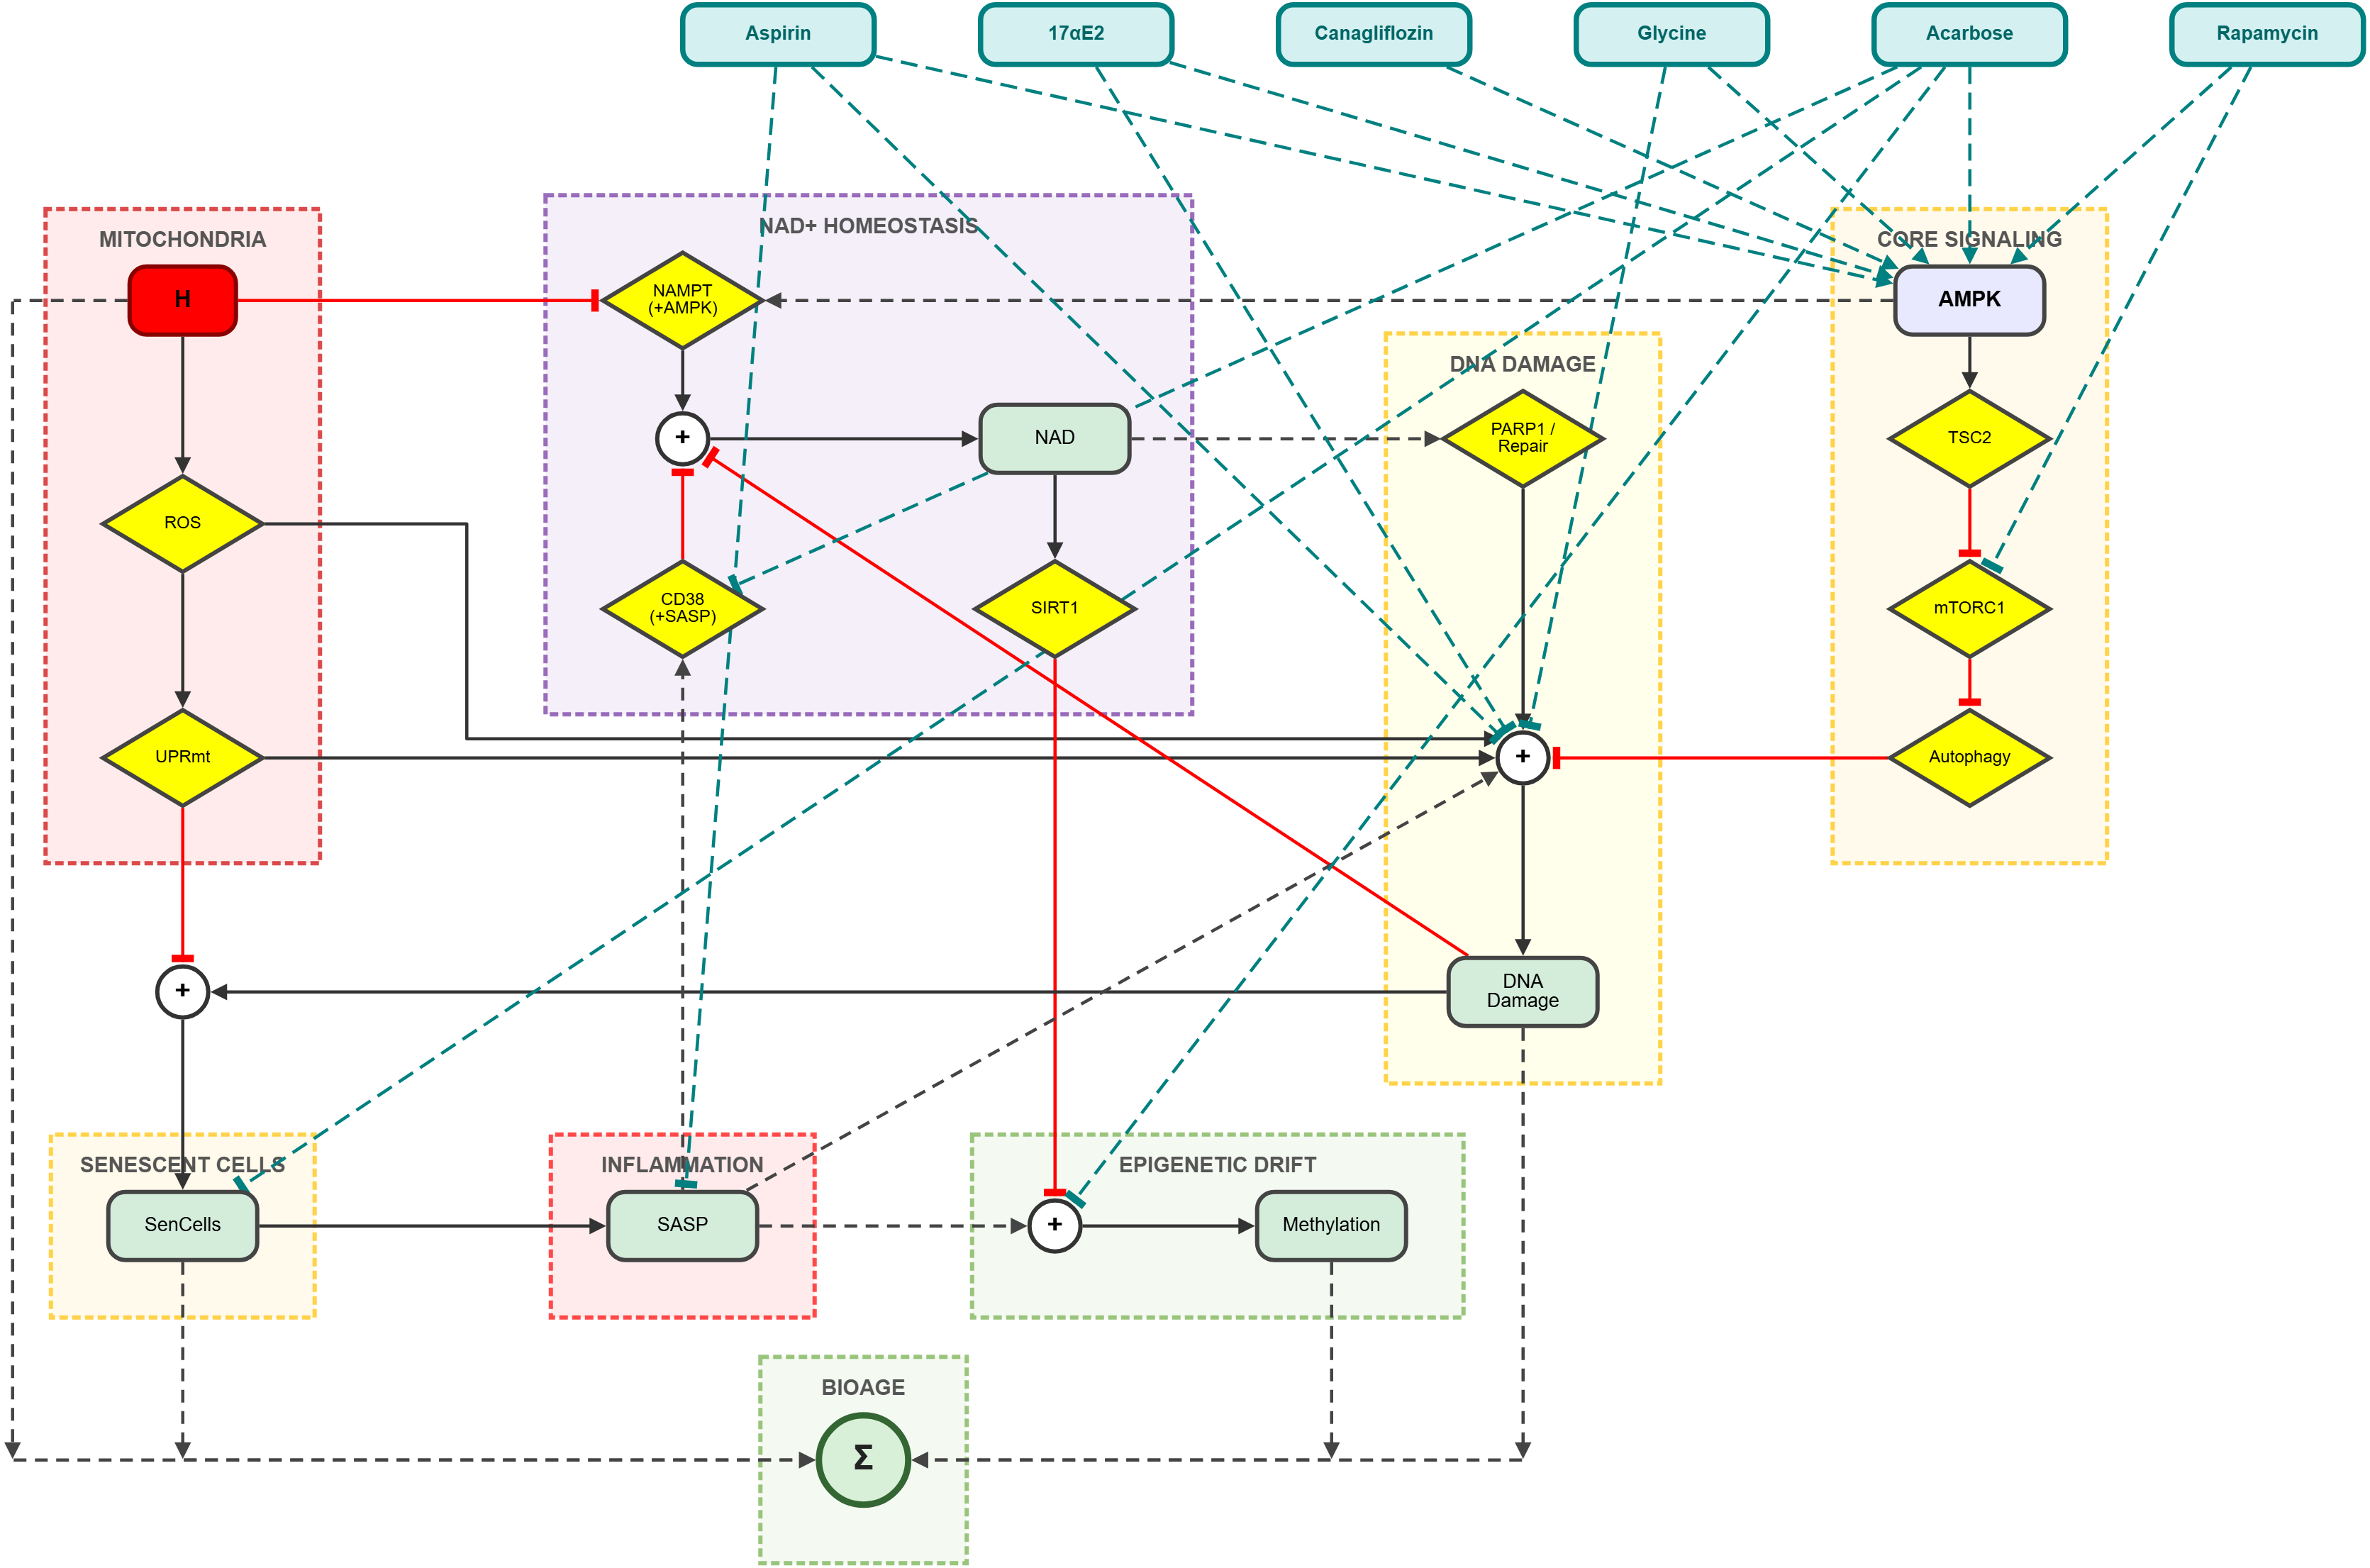
\includegraphics[width=\textwidth]{system_diagram_paper1.png}
\caption{ELM system architecture with ITP compound entry points.}
\label{fig:system}
\end{figure}

\subsubsection{State variables}

Five state variables track the aging subsystems:

\begin{itemize}
\item \textbf{Heteroplasmy} ($H$): fractional mutant mtDNA abundance. $H(0) = 0.011$, meaning 1.1\% of mitochondrial DNA is mutant at birth.
\item \textbf{NAD$^+$ level} ($N$): normalized to young-adult baseline, $N(0) = 1.0$.
\item \textbf{DNA damage} ($D$): normalized double-strand break equivalents. $D(0) = 1.0$, meaning all damage values are measured relative to baseline at birth.
\item \textbf{Senescent cell burden} ($S$): normalized p16$^{\text{Ink4a}}$-positive abundance. $S(0) = 1.0$; senescent cells accumulate above this baseline over the lifespan.
\item \textbf{Methylation drift} ($M$): deviation from youthful CpG set points, $M(0) = 0$.
\end{itemize}

Ten signaling intermediates are computed from the state variables at each time step; they respond instantly, without their own differential equations (Table~\ref{tab:intermediates}). Each is a Hill or Michaelis--Menten function of one or two inputs; for example, SIRT1 activity is $f_{\text{SIRT1}}(N) = N^{n_S} / (K_S^{n_S} + N^{n_S})$, coupling NAD$^+$ levels to downstream deacetylation. They serve as the entry points for compound effects and as the coupling terms between subsystems.

\begin{table}[ht]
\centering
\caption{Signaling intermediates: computed from state variables at each time step (no differential equations of their own).}
\label{tab:intermediates}
\begin{tabular}{@{}llll@{}}
\toprule
Intermediate & Primary inputs & Function type & Key role \\
\midrule
AMPK & energy stress, compounds & Michaelis--Menten & TSC2 activation, NAMPT boost \\
TSC2 & AMPK & Hill ($n = 1.5$) & Rheb-GAP, mTORC1 suppression \\
mTORC1 & TSC2, rapamycin & multiplicative & autophagy inhibition \\
SIRT1 & NAD$^+$ & Hill ($n = 2.0$) & FOXO3 activation, deacetylation \\
FOXO3 & SIRT1 & linear & mitophagy, stress response \\
Autophagy & AMPK, FOXO3 & Michaelis--Menten & damage clearance \\
SASP & SenCells & proportional & CD38, ROS, paracrine senescence \\
ROS & heteroplasmy, SASP & additive & DNA damage source \\
EZH2 & AMPK, SIRT1 & inhibitory & DNMT recruitment, CpG drift \\
PGC-1$\alpha$ & AMPK, SIRT1 & additive & mitochondrial biogenesis \\
\bottomrule
\end{tabular}
\end{table}

\subsubsection{Governing equations}

Heteroplasmy dynamics follow the Kowald--Kirkwood replication advantage model \citep{Kowald1993}:
\begin{equation}
\frac{dH}{dt} = \underbrace{\alpha \cdot H(1 - H)}_{\text{mutant replication advantage}} - \underbrace{\beta \cdot H \cdot \Phi_{\text{mito}}(t)}_{\text{mitophagy clearance}}
\end{equation}
Mutant mtDNA outcompetes wild-type (first term) unless mitophagy removes damaged mitochondria fast enough (second term). $\Phi_{\text{mito}}(t)$ is mitophagy flux, driven by FOXO3 activity.

NAD$^+$ dynamics balance synthesis against three competing drains:
\begin{equation}
\frac{dN}{dt} = \underbrace{k_{\text{synth}} \cdot f_{\text{NAMPT}}(\text{AMPK})}_{\text{NAD$^+$ synthesis}} - \underbrace{k_{\text{PARP}} \cdot D \cdot N}_{\text{DNA repair consumption}} - \underbrace{k_{\text{CD38}} \cdot N}_{\text{CD38 consumption}} - \underbrace{k_{\text{SIRT}} \cdot N \cdot f_{\text{SIRT1}}(N)}_{\text{SIRT1 consumption}}
\end{equation}
The cell makes NAD$^+$ (first term) but three processes consume it: repairing DNA damage, CD38 degradation, and SIRT1 deacetylation. As damage accumulates, the drains win.

DNA damage accumulates from ROS and is repaired by NAD$^+$-dependent pathways:
\begin{equation}
\frac{dD}{dt} = \underbrace{k_{\text{ROS}} \cdot (1 + \gamma_H H + \gamma_{\text{SASP}} \cdot \text{SASP})}_{\text{ROS production, amplified by heteroplasmy \& SASP}} - \underbrace{k_{\text{repair}} \cdot N \cdot D}_{\text{NAD$^+$-dependent repair}}
\end{equation}

Methylation drift is accelerated by damage and SASP, restrained by AMPK-mediated suppression of EZH2, which reduces DNMT recruitment to CpG sites \citep{Vire2006}:
\begin{equation}
\frac{dM}{dt} = k_{\text{drift}}(1 + \delta_D D + \delta_{\text{SASP}} \cdot \text{SASP}) - k_{\text{EZH2}} \cdot f_{\text{AMPK}}(\text{AMPK}) \cdot M
\end{equation}

Senescent cell entry follows a damage-dependent Hill function plus a constant background term $k_{\text{repl}}$ representing replicative exhaustion (Hayflick-limit arrivals per unit time); clearance is proportional to burden:
\begin{equation}
\frac{dS}{dt} = k_{\text{entry}} \cdot \frac{D^n}{K_D^n + D^n} + k_{\text{repl}} - k_{\text{clear}} \cdot S
\end{equation}

\subsubsection{BioAge and survival}

The four damage channels feed into a single number, BioAge, that represents the overall biological age of the mouse. NAD$^+$ is excluded because it acts as a coupling intermediate rather than an independent aging endpoint; its effects are captured through its influence on DNA repair, methylation, and mitophagy:
\begin{equation}
\text{BioAge}(t) = w_H \cdot \frac{H}{\hat{H}_0} + w_D \cdot \frac{D}{\hat{D}_0} + w_M \cdot \frac{M}{\hat{M}_0} + w_S \cdot \frac{S}{\hat{S}_0}
\end{equation}
with equal weights $w_H = w_D = w_M = w_S = 0.25$ (no basis to favor one subsystem over another), where $\hat{H}_0, \hat{D}_0, \hat{M}_0, \hat{S}_0$ are normalization constants derived from control simulation values at $t = 1.0$ (median lifespan), ensuring BioAge$(1.0) = 1.0$ by construction. BioAge determines the death rate through a Gompertz function: $h(t) = h_0 \exp(\lambda \cdot \text{BioAge}(t))$, calibrated to the UM-HET3 control survival curve. We define lifespan extension as the percent change in median survival between treated and control simulations.

The equal-prior weight assignment reflects agnosticism about which subsystem dominates mouse mortality and avoids consuming degrees of freedom on weight tuning. We checked this assumption against three published biological age clocks (GrimAge \citep{Lu2019}, PhenoAge \citep{Levine2018}, DunedinPACE \citep{Belsky2022}) by classifying each clock's biomarkers into ELM subsystems and summing weights per category (Supplementary Table~S13). The clock decomposition does not pin down a unique weight vector, but it does exclude pathological ones: setting $w_M = 0.50$, for example, is outside the range implied by both GrimAge (20--30\%) and PhenoAge (5--15\%). All four equal weights (0.25) fall within every clock's implied range. Sensitivity analysis (Section~3.3) confirms that predictions are stable across the full plausible range.

\subsubsection{Compound implementation}

Each compound perturbs one or more pathway rate constants (Table~\ref{tab:compounds}). An injection value of 0.20 on a pathway means the compound shifts that pathway's activity by 20\% of its dynamic range, from its untreated baseline toward its theoretical maximum effect. A value of 0.42 for rapamycin's mTORC1 inhibition, for example, means rapamycin at the ITP dose pushes mTORC1 42\% of the way from its baseline toward full inhibition.

These values are not set by hand. For each compound, the pharmacological literature establishes which pathways the drug engages. The pathway ratios, how the drug's total effect is divided among its pathways, are estimated from published mechanism-of-action studies: the dominant target receives the largest share. Rapamycin, for example, is assigned 60\% to direct mTORC1 inhibition (its primary target) and 40\% to AMPK activation (a secondary feedback effect). These ratios reflect mechanism hierarchy, not quantitative experimental decomposition; they are constrained estimates, not free parameters, but not directly measured quantities either. Exact values are documented in Supplementary Table~S2.

A single scale factor $\alpha_c$ then sets the overall magnitude: one free parameter per compound, adjusted until the model matches the observed male ITP lifespan extension. The injection value for each pathway equals its share of the split times $\alpha_c$. The resulting values range from 0.03 to 0.42; if the model required most values near 0 or near 1, the pathway assignments would be suspect. The one-at-a-time sensitivity analysis (Supplementary Section~S2.2) confirms that individual ratio perturbations of $\pm$20\% shift predicted lifespan by less than 0.1~pp, so the exact splits do not drive the results.

\begin{table}[ht]
\centering
\caption{Compound pathway assignments and calibrated injection values. For each compound, the pathway \emph{ratios} (column 4) are estimated from mechanism-of-action studies; they encode which pathways the drug engages and in what approximate proportion (Supplementary Table~S2). The \emph{scale factor} $\alpha_c$ (column 5) is the single free parameter per compound, found by root-finding to the male ITP target. The \emph{injection value} (column 6) equals ratio $\times$ $\alpha_c$. Six compounds, six scale factors, six data points.}
\label{tab:compounds}
\begin{tabular}{@{}lllccr@{}}
\toprule
Compound & Mechanism & Pathway & Ratio (lit.) & $\alpha_c$ (fitted) & Injection \\
\midrule
Rapamycin & mTORC1 inhib. & mTORC1 & 0.60 & \multirow{2}{*}{0.70} & 0.42 \\
 & & AMPK & 0.40 & & 0.28 \\
\addlinespace
Acarbose & $\alpha$-glucosidase & AMPK & 0.50 & \multirow{2}{*}{0.34} & 0.17 \\
 & & gut microbiome & 0.50 & & 0.17 \\
\addlinespace
17$\alpha$-Estradiol & 5$\alpha$-reductase & AMPK & 0.50 & \multirow{2}{*}{0.35} & 0.18 \\
 & & antioxidant & 0.50 & & 0.18 \\
\addlinespace
Canagliflozin & SGLT2 inhib. & AMPK & 1.00 & 0.16 & 0.16 \\
\addlinespace
Aspirin & COX inhib. & antioxidant & 0.50 & \multirow{3}{*}{0.20} & 0.10 \\
 & & AMPK & 0.30 & & 0.06 \\
 & & anti-inflam. & 0.20 & & 0.04 \\
\addlinespace
Glycine & antioxidant & antioxidant & 0.90 & \multirow{2}{*}{0.32} & 0.28 \\
 & & AMPK & 0.10 & & 0.03 \\
\bottomrule
\end{tabular}
\end{table}

Three pathways in Table~\ref{tab:compounds} act by modifying rate constants within the existing equations rather than adding new ones. \textbf{Antioxidant} reduces the ROS level in Equation~3: $k_{\text{ROS}}$ is multiplied by a protection factor $(1 - k_{\text{aox}} \cdot \text{antioxidant})$, so glycine's large antioxidant injection (0.28) directly suppresses oxidative DNA damage. \textbf{Gut microbiome} reduces CD38 activity in Equation~2: acarbose's gut fermentation products lower CD38-mediated NAD$^+$ consumption, slowing the $k_{\text{CD38}} \cdot N$ drain term. \textbf{Anti-inflammatory} accelerates SASP clearance, reducing the SASP-driven amplification terms that appear in Equations 2, 3, and 4. All three pathways modify rate constants within the existing ODE structure rather than adding new equations.

\subsection{Calibration}

We calibrate the model with one free parameter per compound: a scale factor $\alpha_c$ that we adjust (via root-finding) until the predicted male lifespan extension exactly matches the ITP observation:
\begin{equation}
\Delta L_{\text{pred}}^{(c, \text{male})} = \Delta L_{\text{ITP}}^{(c, \text{male})}
\end{equation}
Male predictions are exact by construction (error $< 0.01$~pp). 162 additional parameters are fixed before calibration begins: 115 from published experimental measurements, 24 set within biologically plausible ranges (including 6 adjusted to produce realistic untreated-mouse biology), and 23 structural constants (normalization, coupling topology). None were adjusted to match ITP intervention outcomes. Full provenance is documented in the Supplementary Material.

We then compute female predictions using the same scale factors plus the four sex-specific mechanisms. No parameters are adjusted to match female data. These are genuine out-of-sample predictions.

\subsection{Sex-Specific Implementation}

\textbf{AMPK saturation.} Female AMPK baseline is $b = 1.3\times$ male \citep{Boudaba2018,McInnes2011}. We model this saturation as $f_{\text{atten}} = 1/(1 + k(b - 1))$ with $k = 8$, giving a factor of 0.29, meaning females get roughly one-third of the AMPK-mediated benefit that males get. This single functional form governs female response for all three AMPK-activating compounds (acarbose, canagliflozin, glycine).

\textbf{CYP3A pharmacokinetics.} Female effective rapamycin exposure is $3.48\times$ male \citep{Lamming2014}, applied via Hill-function mTORC1 inhibition.

\textbf{Testosterone dependency.} 17$\alpha$-estradiol perturbation is set to zero in female simulations \citep{Garratt2018}.

\textbf{COX-2 interference.} A PGI$_2$ offset cancels aspirin's antioxidant benefit in females \citep{Egan2004,Grosser2006}.

\subsection{Combination Simulation}

In combination simulations, we activate both compound perturbations at once, each applied to its own rate constants. Cross-compound interactions arise only through shared state variables. The rapamycin + acarbose combination was simulated from a 9-month start time matching the ITP protocol \citep{Strong2022}.

\subsection{Sensitivity Analysis}

We varied each BioAge weight across $[0.10, 0.50]$, redistributing the remainder equally, and recalibrated the model at each value. We independently perturbed each compound scale factor $\pm$20\%.\footnote{ODEs were integrated with SciPy \texttt{solve\_ivp} (RK45). All code is available at \url{https://github.com/silmonbiggs/extensible-longevity-model} (MIT license).}

% ============================================================
\section{Results}
% ============================================================

\subsection{Sex Differences: Four Mechanisms, Zero Sex-Specific Fitting}

Using four biological mechanisms drawn from prior literature, none fitted to female data, the model predicts all six female ITP outcomes from male calibration alone, with 1.3~pp mean absolute error (median 0.45~pp; Table~\ref{tab:calibration}). This is the primary result.

\begin{table}[ht]
\centering
\caption{ITP observed vs.\ ELM predicted lifespan extension. Male predictions are calibrated (6 free parameters); female predictions are genuine out-of-sample tests.}
\label{tab:calibration}
\begin{tabular}{@{}l|cc|cc|l@{}}
\toprule
 & \multicolumn{2}{c|}{\textbf{Male (calibrated)}} & \multicolumn{2}{c|}{\textbf{Female (predicted)}} & \\
Compound & ITP & ELM & ITP & ELM & Sex mechanism \\
\midrule
Rapamycin      & +23.0\% & +23.0\% & +26.0\% & +26.7\% & CYP3A pharmacokinetics \\
Acarbose       & +22.0\% & +22.0\% & +5.0\%  & +7.6\%  & AMPK saturation \\
17$\alpha$-Estradiol & +19.0\% & +19.0\% & 0\%     & 0\%     & testosterone dependency \\
Canagliflozin  & +14.0\% & +14.0\% & +9.0\%  & +5.0\%  & AMPK saturation \\
Aspirin        & +8.0\%  & +8.0\%  & 0\%     & 0\%     & estrogen interference \\
Glycine        & +6.0\%  & +6.0\%  & +4.0\%  & +3.8\%  & AMPK saturation \\
\bottomrule
\end{tabular}
\end{table}

\textbf{AMPK saturation (acarbose, canagliflozin, glycine).} A 30\% higher AMPK baseline, on a steeply saturating curve, leaves only 29\% of the male drug response available (attenuation factor 0.29). The per-compound predictions: glycine is predicted well (+3.8\% vs.\ +4.0\%), acarbose is overpredicted (+7.6\% vs.\ +5.0\%), and canagliflozin is underpredicted (+5.0\% vs.\ +9.0\%).

The acarbose--canagliflozin error pattern is diagnostic. If both compounds acted purely through AMPK, their female attenuation should be similar. Instead they err in opposite directions: acarbose is overpredicted, canagliflozin is underpredicted.

The most parsimonious explanation: canagliflozin has a second, sex-independent mechanism, possibly FGF21/ketogenesis via SGLT2 inhibition, that the single-AMPK model does not capture. Three independent lines of evidence support this: SGLT2 inhibition shifts substrate utilization toward fatty acid oxidation and ketogenesis \citep{Ferrannini2016}; canagliflozin specifically reprograms systemic metabolism via FGF21-dependent pathways in mice \citep{Osataphan2019}; and SGLT2 inhibitors activate ketogenic starvation sensors independently of glucose lowering \citep{Packer2020}. This is a hypothesis the model generates, not one it was designed to test.

\textbf{Pharmacokinetics (rapamycin).} Rapamycin is the one compound showing greater female efficacy (+26\% F vs.\ +23\% M). The AMPK saturation mechanism predicts the opposite. The reversal is pharmacokinetic: female mice achieve 3.48-fold higher blood rapamycin levels at equivalent dietary doses due to reduced CYP3A hepatic clearance \citep{Lamming2014}, more than offsetting the AMPK disadvantage. The model predicts +26.7\% female, an error of 0.7~pp.

\textbf{Testosterone dependency (17$\alpha$-estradiol).} Without testosterone substrate, the mechanism is inoperative in females, confirmed experimentally in castrated males, which lose efficacy entirely \citep{Garratt2018}. Predicted: 0\%. Observed: 0\%.

\textbf{Estrogen interference (aspirin).} COX inhibition suppresses the COX-2$\to$PGI$_2$ pathway through which estrogen mediates cardioprotection \citep{Egan2004,Grosser2006}. The net effect in females neutralizes a protective pathway, offsetting aspirin's antioxidant and anti-inflammatory benefits. Predicted: 0\%. Observed: 0\%.

No sex-specific parameters were adjusted to ITP lifespan data. The AMPK baseline ratio (1.3$\times$) and rapamycin PK ratio (3.48$\times$) come from published measurements; the saturation curvature ($k = 8$) is a round number set near the midpoint of the plausible range [3--20] (Section~4.2). All three were fixed before examining female ITP outcomes.

\begin{figure}[H]
\centering
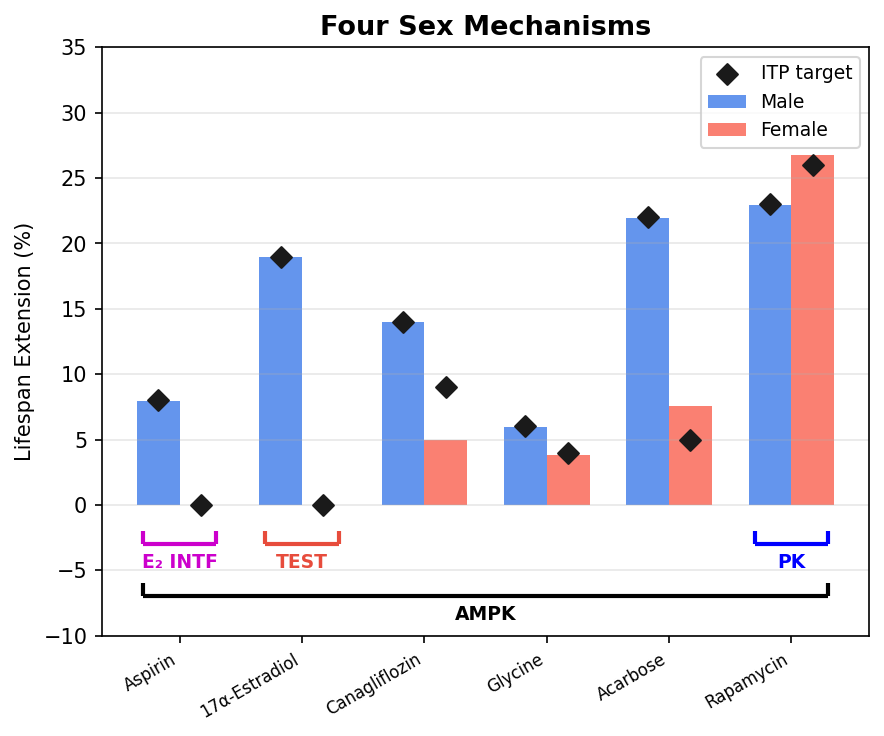
\includegraphics[width=0.85\textwidth]{stage_11_mf_complete.png}
\caption{Sex difference predictions vs.\ ITP observations for all six compounds.}
\label{fig:sex_diff}
\end{figure}

Figure~\ref{fig:rapa_survival} shows predicted survival curves for rapamycin-treated and control mice in both sexes. In males, rapamycin shifts the survival curve rightward by a modest margin; the two curves separate gradually. In females, the separation is visibly larger: higher effective drug exposure (3.48$\times$ blood levels) pushes the treated curve further right, producing a larger gap at every survival quantile. The model captures this asymmetry from the CYP3A pharmacokinetic difference alone, without any female-specific fitting.

\begin{figure}[H]
\centering
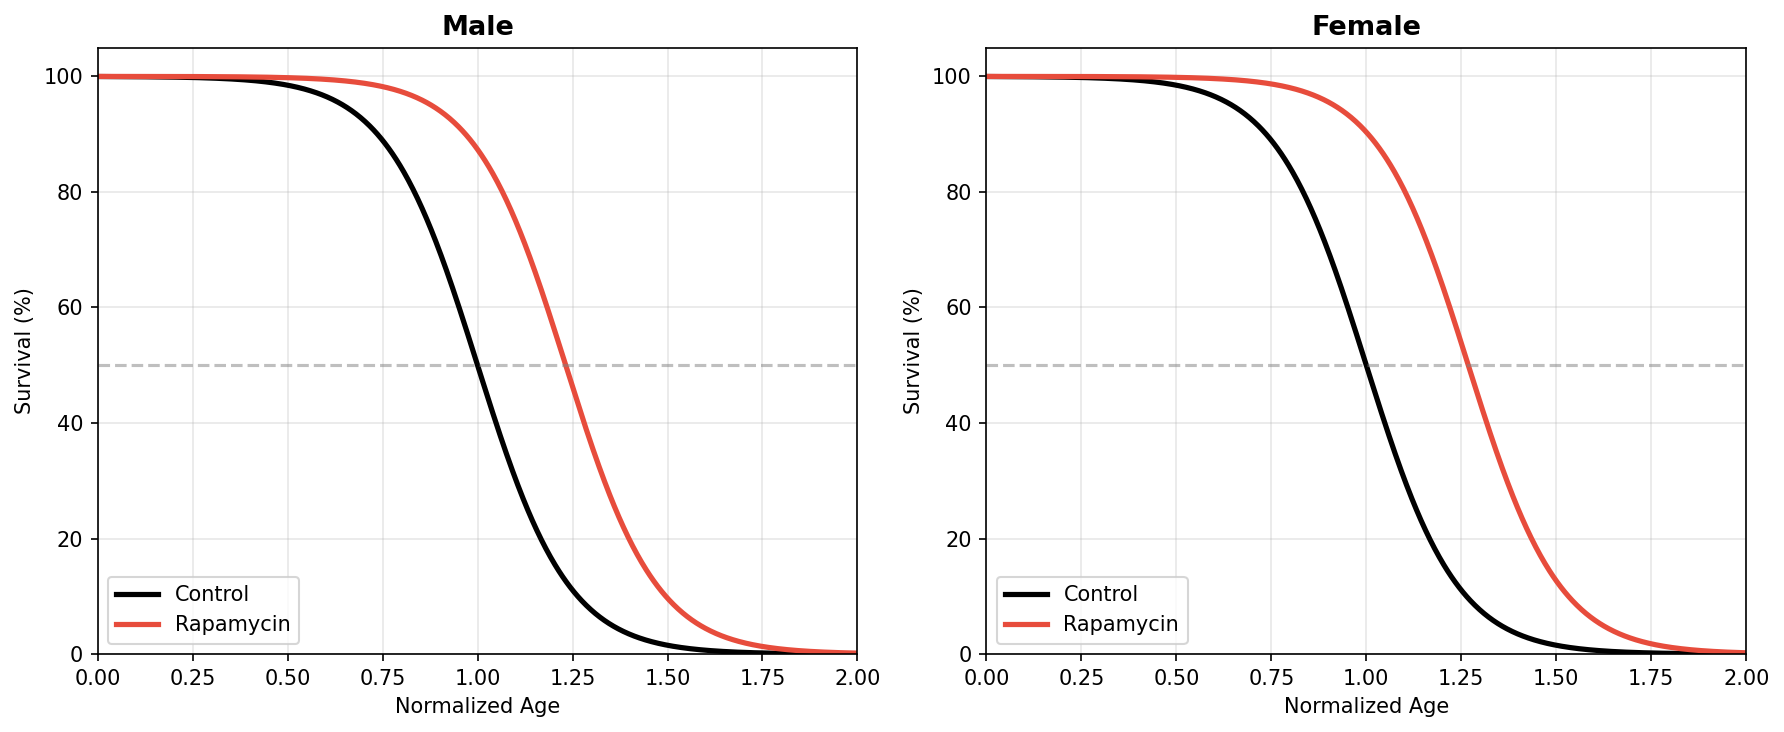
\includegraphics[width=\textwidth]{rapa_survival_mf.png}
\caption{Predicted survival curves for rapamycin-treated (red) vs.\ control (black) mice. Left: males (+23\%). Right: females (+26.7\%). The larger female separation reflects 3.48$\times$ higher effective drug exposure from reduced CYP3A hepatic clearance.}
\label{fig:rapa_survival}
\end{figure}

\subsection{Out-of-Sample Validation: Rapamycin + Acarbose}

The ELM predicts +33.5\% for the rapamycin + acarbose combination; the ITP observed +34\% \citep{Strong2022}. This combination was not used in any parameter fitting: neither the compound scale factors (calibrated to individual male targets) nor the BioAge weights (equal priors, fixed before calibration) were adjusted to match this result.

The prediction is not trivially correct. Both compounds activate AMPK, but through different routes: rapamycin indirectly (mTORC1 inhibition relieves negative feedback on AMPK) and acarbose directly (energy stress from reduced carbohydrate absorption). Both converge on the same downstream autophagy pathway, which follows Michaelis--Menten kinetics with $K_a = 0.35$.

At ITP doses, rapamycin alone drives autophagy to $\sim$78\% of maximum; acarbose drives it to $\sim$65\%. Combined, the pathway encounters diminishing returns near saturation. A naive additive model predicts +45\%. The ELM predicts +33.5\%. The ITP observes +34\% (Figure~\ref{fig:combo}). The naive model is not close. The ELM identifies the direction of the interaction (sub-additive), its approximate magnitude, and the correct mechanistic reason: pathway saturation at a shared node.

\begin{figure}[H]
\centering
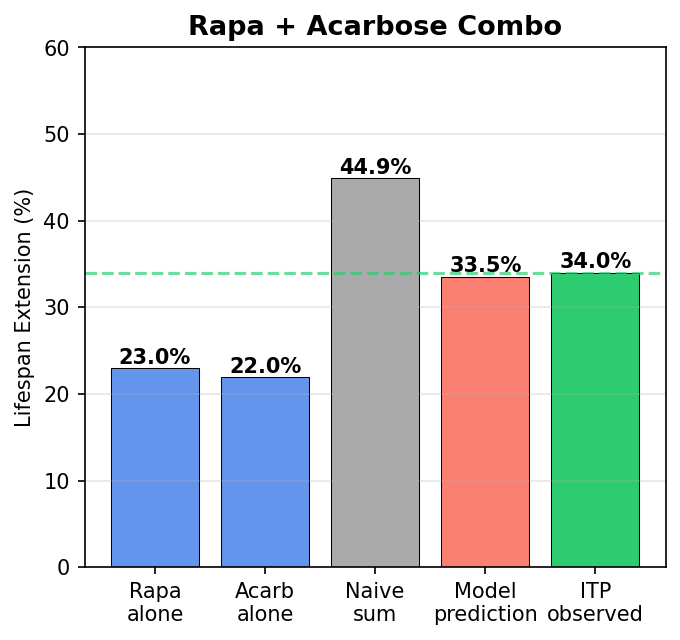
\includegraphics[width=0.6\textwidth]{stage_08_mixing_bars.png}
\caption{Out-of-sample combination prediction: rapamycin + acarbose.}
\label{fig:combo}
\end{figure}

\subsection{Sensitivity and Robustness}

\textbf{Weight sensitivity.} We swept the methylation weight across $[0.05, 0.50]$, well beyond the biologically plausible clock-decomposition range of $[0.05, 0.30]$ (Supplementary Section~S3). Across the full sweep, the combination prediction ranges from +31.0\% ($w_M = 0.05$) to +37.3\% ($w_M = 0.50$). Within the plausible range, the combination prediction spans +31.0\% to +34.3\% and the female mean error spans 1.20 to 1.36~pp---the model is insensitive to this weight across its plausible range (Figure~\ref{fig:weight_sweep}).

\textbf{Parameter perturbation.} Perturbing each compound scale factor $\pm$20\% shifts individual predictions by at most 2~pp. No perturbation reverses any sex-difference direction or changes the qualitative combination prediction.

\textbf{Background aging rate test.} If the model were just rescaling a single aging rate, then changing any one parameter would shift all predictions by the same fraction. We tested this by increasing the heteroplasmy replication advantage by 10\%: all 12 predictions shift, but by different amounts (ratios ranging from 0.151 to 0.207, a 37\% spread). The model is not a disguised one-parameter fit.

\begin{figure}[H]
\centering
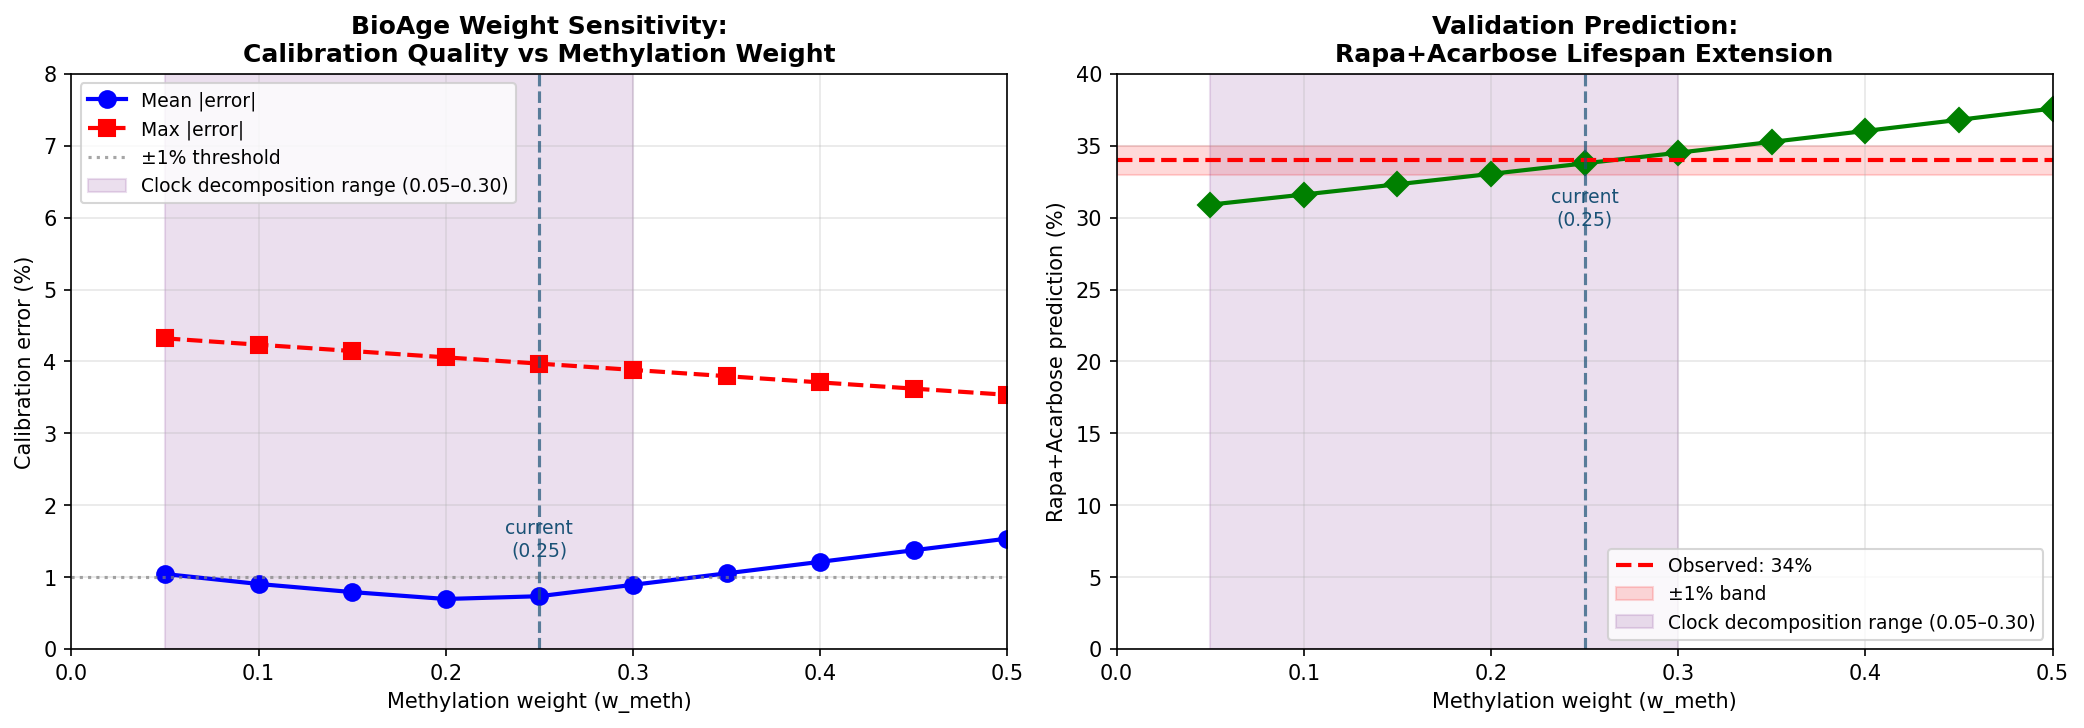
\includegraphics[width=\textwidth]{w_meth_sweep.png}
\caption{BioAge weight sensitivity: calibration quality and combination prediction.}
\label{fig:weight_sweep}
\end{figure}

% ============================================================
\section{Discussion}
% ============================================================

\subsection{The Sex Difference Explanation}

No single mechanism here is new; each has been proposed before. What is new is that four independent mechanisms, drawn from four different literatures, all produce correct predictions when combined in the same quantitative model. That all four produce correct directional predictions, and four of six within 1~pp, is evidence that the model captures real biology.

The canagliflozin error pattern suggests a specific experimental test. The model underpredicts female canagliflozin efficacy (+5.0\% vs.\ +9.0\%) because it routes the entire effect through AMPK, which is heavily attenuated in females. If canagliflozin also acts through a second pathway (FGF21/ketogenesis, for which there is independent literature support \citep{Ferrannini2016,Osataphan2019,Packer2020}) and if that pathway is sex-independent (not subject to AMPK saturation), then females would retain that component unattenuated, raising the predicted female benefit toward the observed value. The test: measure FGF21 levels in canagliflozin-treated male and female mice. If FGF21 rises equally in both sexes, it confirms the multi-pathway hypothesis and indicates that adding this second pathway to the model would resolve the prediction error.

\subsection{The Combination Validation}

The rapamycin + acarbose prediction (+33.5\% vs.\ +34\%) provides supporting evidence beyond the sex differences. Its value lies in what the model had to get right: predicting sub-additivity rather than the naive +45\%, for the correct mechanistic reason. But one combination prediction does not validate the full model; it validates the specific pathway saturation mechanism that both compounds share. The harder test, cross-pathway interactions involving mechanistically independent axes, requires multi-compound experimental designs that have not yet been conducted, because single-compound testing, however rigorously conducted, cannot see what is behind a wall it has not yet removed.

\subsection{What the Data Constrains}

The model has 6 calibrated parameters and 162 frozen priors: 115 from published measurements, 24 set within biologically plausible ranges, and 23 structural constants. It is a 6-parameter model that has imported a large body of experimental biology as fixed assumptions. The model predicts correctly not despite its enormous null space but because of it: the null space is where the priors live, and those priors, whether measured directly, constrained by published biology, or set at plausible midpoints, are the best information presently available. But the priors are not all equally right. The edges of that imported knowledge are where the model will fail first. One-at-a-time sensitivity analysis of all 141 perturbable frozen priors is provided in the Supplementary Material (\S S2.2).

\subsection{Downstream Predictions}

Beyond the sex differences and combination validation reported here, the model generates predictions about multi-compound interventions. The most striking: when the four best ITP compounds are combined, the model predicts that mitochondrial heteroplasmy becomes the dominant remaining cause of aging-related death---rising from 25\% to 40\% of biological age at death. The reason is simple: no ITP compound directly targets mitochondrial DNA quality control. The remaining modes do not vanish; they wait. This implies that the next large gain requires addressing a different aging axis entirely. These predictions, with novel target rankings and specified falsification conditions, are reported separately (Biggs 2025, preprint).

\subsection{Limitations}

\textbf{Cross-pathway independence.} The central unvalidated assumption is that the four aging axes compound approximately independently in living animals. The ODE coupling structure encodes known interactions (SASP$\to$NAD$^+$ drain, ROS$\to$DNA damage, AMPK$\to$EZH2 methylation), but the model assumes these are the dominant cross-pathway interactions. Higher-order feedback not captured in the system could invalidate combination predictions.

\textbf{AMPK saturation parameter.} The diminishing-returns curvature $k = 8$ is a modeling choice, not a directly measured quantity. It is set as the midpoint of the plausible range for hyperbolic saturation of the LKB1$\to$AMPK$\to$TSC2 cascade. Different values of $k$ shift the three AMPK-compound female predictions in concert; the qualitative pattern (acarbose overpredicted, canagliflozin underpredicted) is preserved across the plausible range.

\textbf{Scope.} The model does not include Wnt/$\beta$-catenin, Notch, telomere dynamics, immune senescence, AGE crosslink accumulation, or organ-specific fibrosis. It makes no quantitative claims about human outcomes. These are targets for future extension of the model. The ODE architecture is modular: each subsystem couples to the others only through named signaling intermediates, so new subsystems can be added without refitting the existing structure, as long as the new module says how it connects to the rest.

\subsection{Relationship to Existing Models}

No individual equation in ELM is new; each draws on reliability theory \citep{Gavrilov2001}, mechanistic aging models \citep{Kowald1993,Kogan2015,Podolskiy2015}, and the hallmarks framework \citep{LopezOtin2013,LopezOtin2023}. What is new is the combination: calibration to ITP lifespan data, prospective out-of-sample validation against ITP sex data, and specified falsification conditions. To our knowledge, prior models in this space have not been calibrated to ITP data or validated prospectively on unseen outcomes, which raises a question about what, exactly, they are predicting. A model that cannot be wrong is not a model; it is a metaphor.

\subsection{Conclusions}

A 6-parameter model, calibrated only to male ITP data, predicts all six female outcomes with 1.3~pp mean absolute error (median 0.45~pp) using four independently motivated sex mechanisms---and predicts the rapamycin + acarbose combination with 0.5~pp error, for the correct mechanistic reason. Where it errs, it points to a testable hypothesis: canagliflozin has a second pathway the model does not yet capture.

% ============================================================
% Bibliography
% ============================================================

\bibliographystyle{unsrtnat}
\bibliography{references}

\end{document}
